\chapter[LWFA Bremsstrahlung Source for linear BW]{Characterisation of a LWFA Bremsstrahlung Source for a Measurement of the Linear Breit-Wheeler Process}
\label{Chap:BW}

\section{Motivation and Introduction}

The Breit-Wheeler process \cite{BreitWheeler1934_BW} is the inverse process of the more commonly observed Dirac annihilation \cite{Dirac1930_Annihilation}, where an electron and a positron decay into two photons. In the Breit-Wheeler mechanism, two (linear) or more (non-linear) photons combine to produce an electron-positron pair --- in other words matter is created from light. The linear Breit-Wheeler process is the simplest mechanism by which photons can create matter and is one of the most fundamental interactions of quantum electrodynamics (QED) that can be represented by minimally-sized Feynman diagrams (see Figure \ref{BW:Figs:OPike_TreeDiagrams}). However, despite its simplicity it is the last of these fundamental interaction that has not been definitively observed in isolation in vacuum, i.e. without the presence of other particles or external fields. Its measurement is particularly relevant for the field of high-energy astrophysics \cite{Nikishov1962_PAIRSASTRO,Bonometto1971_PAIRSASTRO,Ruffini2010_PAIRSASTRO}.
\vspace{\baselineskip}

The non-linear Breit-Wheeler process, on the other hand, has been measured and confirmed previously as part of the E144 experiment at SLAC in the `90s where an ultrarelativistic electron beam of $46.6\,\mathrm{GeV}$ energy was collided with an intense laser pulse $a_0 \sim 0.3$, resulting in highly energetic gamma photons from inverse Compton scattering \cite{Bula1996_RR,Burke1997_RR}. These gamma photons in turn interacted with up to $n \approx 7$ laser photons to produce electron-positron pairs \cite{Hu2010_TRIDENT}. The researchers detected about 100 positrons that match the momentum profile for products from the non-linear Breit-Wheeler and the Trident process \cite{Ilderton2011_TRIDENT} over the course of 22,000 laser shots.

The measurement of other photon-photon interactions, elastic and inelastic scattering processes, is additionally very challenging as these are higher order processes with cross sections that are suppressed by at least $\sim \alpha^{-2}$. As a result similarly few events have been measured for other photon-photon interactions without background fields, for instance at the Large Hadron Collider (LHC): the ATLAS collaboration reported on 13 candidate events for light-light scattering in heavy-ion collisions \cite{ATLAS2017_GammaGamma,dEnterria2013_GammaGamma}. The OPAL Collaboration at LEP, on the other hand, measured inelastic photon-photon interactions \cite{OPAL2000_GammaGamma}.
\vspace{\baselineskip}

\begin{figure}
\centering
\includegraphics[width=.9\columnwidth]{QED_TreeDiagrams_OPike.jpg}
\caption[Overview of theoretical fundamental QED processes shown in their Feynman representation along with the year the process was validated experimentally.]{Overview of theoretical fundamental QED processes shown in their Feynman representation along with the year the process was validated experimentally. Each of the processes has been observed in experiment, with exception of the Breit-Wheeler pair production, and either theoretical or experimental work related to them has been rewarded with a Nobel prize. Figure by Oliver Pike, accessible at \cite{Pike_PHYSORG}}%https://phys.org/news/2014-05-scientists-year-quest.html
\label{BW:Figs:OPike_TreeDiagrams}
\end{figure}

Pair annihilation is easily measured in radioactive decays \cite{Klemperer1934_Annihilation} as its cross section is very high at low energies ($\sigma_{e^+ e^-} \propto 1/E$) and an abundance of electrons in ordinary matter provides an abundance of attractive partners for positrons to annihilate with. Pair creation from radiation, on the other hand, requires high energy photons and/or a very high photon density, for instance a tightly focused laser, to overcome the production threshold in the centre-of-mass frame:

\begin{equation}
\boxed{s = \frac{E_1 E_2}{2m^2_e c^4} (1-\cos\theta) > 1,}
\end{equation}

where $s$ is the centre-of-mass energy, $E_1,E_2$ the energy of the first and second photon, respectively, and $\theta$ is the angle between the two photons.
Any excess energy can provide the created pair with sufficient momentum to avoid an immediate decay through Dirac annihilation. The quantities of the Breit-Wheeler and annihilation total cross-sections are related by $\sigma_{\gamma \gamma} = 2\beta^2 \sigma_{e^+e^-}$, where $\beta = \sqrt{1-1/s}$ (see Figure \ref{BW:figs:BW_Dirac_Xsec}).
However, delivering two bright energetic photon sources at suitable energies at the same location is very challenging and hence mainly mediated pair production processes in presence of a background field have been measured instead \cite{Bethe1934_BH,Heitler1954_BH,Gahn2000_BH,Chen2009_BH,Sarri2013_pairs,Sarri2015_pairs,Bula1996_RR}. 
\vspace{\baselineskip}

\begin{figure}
\centering
\includegraphics[trim={5.0cm 0 6.0cm 0}, clip, width=1.0\columnwidth]{BWD_Xsec.png}
\caption[Breit-Wheeler and Dirac cross-section.]{Breit-Wheeler and Dirac cross section as function of the centre-of-mass energy $\sqrt{s}$. For $s\rightarrow 1$ the pair production cross section falls to zero whilst the annihilation cross section diverges. The maximum value of the Breit-Wheeler cross section coincides with the energy at which both cross sections are equal.}
\label{BW:figs:BW_Dirac_Xsec}
\end{figure}

Directed high energy radiation in the $\mathrm{keV}$ range can be produced from highly relativistic electrons, for instance at XFELs and synchrotron sources using bending magnets and insertion devices, and equivalently in plasma accelerators through betatron radiation \cite{Rousse2004_BETATRON,Kneip2010_BETATRON}. Another approach is to heat solid targets with a laser, for instance hohlraums \cite{PikeThesis} or burn-through foils \cite{Edwards1990_BURNTHROUGH}.

Directed energetic gamma radiation can be generated by passing highly relativistic electrons through solid material to produce bremsstrahlung \cite{Glinec2005_Brems} or relying on inverse Compton scattering \cite{Sarri2014_ICS,Yan2017_ICS}.
\vspace{\baselineskip}

\begin{figure}
\centering
\includegraphics[width=.7\columnwidth]{OPike_nphoton_plot.JPG}
\caption[Experimental setup for a photon-photon collider as proposed by Pike et al.]{Experimental setup for a photon-photon collider to produce and measure pair production from the linear Breit-Wheeler process as proposed by Pike et al. in \cite{Pike2014_BW}. From left to right: an electron beam (grey circles with black momentum arrows) from a laser wakefield accelerator is incident on gold target and produces gamma-ray photons (red, blue and purple wave packets) from bremsstrahlung. The remaining electrons and electron-positron pairs produced in the interaction with the solid are removed from the system using a dipole magnet. The gamma-ray photons enter the blackbody radiation field (red) generated by heating a hohlraum (gold). In the interaction of the gamma-rays and the radiation field electron positron pairs (grey) are produced and emitted in the propagation direction of the gamma-rays. The pairs are dispersed by a magnetic field and directed onto suitable detectors (not shown). This is Figure 1 in \cite{Pike2014_BW} reprinted by permission from Nature Photonics, copyright (2019).}
\label{BW:figs:PikeSetup}
\end{figure}


In 2014, \textit{Pike et al.} \cite{Pike2014_BW} proposed to measure the linear Breit-Wheeler process by combining a low-divergence ($\theta \sim \ln(\gamma)/\gamma$ \cite{Stearns1949_Brems}) bremsstrahlung source, consisting of a GeV-class electron beam generated by a high-intensity laser\cite{Leemans2006_GEV}  and a gold foil \cite{Glinec2005_Brems}, with a blackbody radiation field formed in a hohlraum heated by a high-energy laser (see Figure \ref{BW:figs:PikeSetup}) \cite{Lindl2004_HOHLRAUMBASICS,Decker1997_HOHLRAUM,Town2011_HOHLRAUM,Glenzer2011_HOHLRAUM}. For $10^9$ electrons at 2 GeV energy, a 5 mm thick gold foil and a 1-cm long hohlraum at temperature of 400 eV, the researchers predicted up to $10^5$ pairs to be generated from the linear Breit-Wheeler process. The asymmetry of the energies produced by the two photon sources results in an emission of pairs in the direction of the higher energetic gamma ray beam. This is referred to as pair beaming \cite{Ribeyre2018_BW}, which in principal allows the extraction and measurement of all pairs produced, better separation of signal and noise, and using smaller detectors.
The setup also opens up the possibility to investigate elastic photon-photon scattering of the gamma-rays in the X-ray field \cite{dEnterria2013_GammaGamma}.

\begin{figure}
\centering
\includegraphics[width=.7\columnwidth]{2018QED_Chicane.JPG}
\caption[In pursuit of creating matter from light. Photograph of the magnetic chicane.]{In pursuit of creating matter from light. Photo taken during the experiment campaign aimed at measuring the linear Breit-Wheeler process at the Gemini facility in 2018. View upstream on the gamma-ray axis, indicated by a green alignment laser, through the magnetic chicane that is designed to transport generated electron-positron pairs from the Breit-Wheeler process to designated single particle detectors.}
\end{figure}

The experiment presented here is based on this proposed layout \cite{Pike2014_BW,PikeThesis}: two lasers are employed to provide simultaneously an X-ray and a gamma-ray source to overcome the mass threshold and to produce electron-positron pairs from the linear Breit-Wheeler process. A detailed description can be found in Section \ref{BW:sec:expSetup} (see also Figure \ref{BW:fig:exp_sketch}). The gamma rays are produced, as proposed, by bremsstrahlung from LWFA electrons \cite{Glinec2005_Brems}, but in this instance typically at electrons energies $\epsilon_{e^-} < 1\,\mathrm{GeV}$. As converter the higher-Z metal bismuth (Bi) is used which allows reducing the material thickness with respect to the proposed gold foil at comparable conversion efficiency, but at lower maximum cut-off energy due to the lower electron energies. Instead of using a high-energy laser and a hohlraum, a replenishable germanium target is used as burn-through foil germanium target in conjunction with another high-intensity laser \cite{Edwards1990_BURNTHROUGH}, producing an X-ray spectrum with emission lines peaked around $1.5\,\mathrm{keV}$ \cite{Roberts1980_AWECODE}. This balances out the lower gamma-ray energy and a narrow bandwidth spectrum constrains the interaction conditions.
Using a replenishable foil target and a high-intensity instead of a high-energy laser also allows making use of high repetition rate systems.
By removing the X-ray target from the beam axis we also reduce the production of secondary Bethe-Heitler pairs \cite{Bethe1934_BH} from gamma rays interaction with solids that might be mistaken for pairs produced in the linear Breit-Wheeler process.

\section{Chapter Outline}

This Chapter relates to an experimental campaign aimed at measuring the linear Breit-Wheeler process \cite{BreitWheeler1934_BW} conducted at the Gemini laser system in spring 2018. Two high-intensity lasers are used to provide provide a highly energetic gamma radiation and an X-ray source that combined exceed the production threshold of a centre-of-mass energy of $s > 1$.

The experiment can be divided in three major components: the gamma-ray source, the X-ray source and the single-particle detectors.

This work focuses on the commission, characterisation and considerations related to the gamma-ray source. This is the main contribution of the author to the overall analysis of the experimental data.
In some parts, this Chapter will refer to analysis from diagnostics related to the other two areas where the author has not directly contributed to the analysis itself. 
The X-ray data has been analysed by Cary Colgan (Imperial College) and Brendan Kettle (Imperial College), with John Morton (AWE) providing simulations for the X-ray spectra. Data related to the single particle detectors has been analysed by Brendan Kettle (Imperial College) and Guillermo Marrero Samarin (QUB) with significant contribution from Dominik Hollatz (Jena) for the tracking of particles through the magnetic chicane.
\vspace{\baselineskip}

In this experiment, the gamma-ray source is generated by bremsstrahlung from LWFA electrons traversing a solid target \cite{Glinec2005_Brems}.
The properties of the electrons determine the properties of the radiation produced, but LWFA electrons underlie intrinsic fluctuations and properties vary from experiment to experiment (REF). Hence, the electron properties are first characterised in general and more specifically its variation in performance for three relevant shot days. The primary properties of interest are charge, electron energy, divergence and the stability of the shot-to-shot beam pointing.
The properties of radiation that the electron beam produces are investigated for two different density regimes of the accelerator and two converter materials at two different thicknesses. The performance of the source in its different configurations is analysed and optimised in terms of yield enclosed within a certain divergence angle and the signal-to-noise ratio registered on the single-particle detectors.
Using the optimised parameters for the bremsstrahlung source, the performance and the fluctuations of the gamma source are characterised for the three shot days. 

Then, the measured spectra of the X-ray source, analysed by Cary Colgan (Imperial College), and its performance for the shot days are presented.

Combining the characterisation of the gamma-ray source and the X-ray source the impact of the varying performance of both on the total Breit-Wheeler cross section for the three shot days is analysed and discussed.

To provide the context and significance of this Chapter, a brief overview of the overall analysis is given.

Finally, the results are summarised and potential improvements for a future measurement are discussed.

\section{Experimental Setup}
\label{BW:sec:expSetup}

The experiment was performed at the dual 300 TW Ti:Sa Gemini laser at the Central Laser Facility, UK, in early 2018.
The aim of this setup was to produce and to measure electron-positron pairs from the linear Breit-Wheeler process \cite{BreitWheeler1934_BW}. For this purpose, high-energy bremsstrahlung gamma-rays produced by LWFA electrons \cite{Glinec2005_Brems} were collided with X-rays from a heated burn-through foil \cite{Edwards1990_BURNTHROUGH}. The first laser of the Gemini laser provided the X-rays, the second laser the gamma source.

A sketch of the experimental setup is shown in Figure \ref{BW:fig:exp_sketch}.

\begin{sidewaysfigure}
\centering
\includegraphics[width=1.0\columnwidth]{BW2018_render_V4_annotated.png}%{BW2018_render_V3_annotated3.png}
\caption[Sketch of the experimental setup for the Breit-Wheeler campaign.]{Sketch of the experimental setup indicating its main components. From left to right: The first laser pulse (left, red) is focused by an $f/40$ OAP into a gas cell target (blue), producing an electron beam (blue) via LWFA leaving the cell on the right side. The remainders of the laser pulse are removed after the cell by a kapton tape acting as plasma mirror (orange). The electron beam passes through the tape traverses a metal converter target producing gamma radiation from bremsstrahlung (green) in forward-direction. A tungsten (W) collimator removes the divergent components of the radiation and a thick W block shields the direct line of sight to the X-ray target further downstream. When the converter (and the collimator) are not in the path of the electron beam, it is characterised by a magnetic spectrometer using a permanent dipole magnet. A second laser (red) is focused onto a kapton tape with germanium (Ge) dots (orange) act as source of X-rays (green) that are characterised by a crystal spectrometer and a pinhole camera (turquoise). Positrons produced in the interaction of the X-rays and gamma-rays propagate downstream and are directed through a magnetic chicane and onto single particle detectors (brown). The gamma-rays are measured by a gamma profile detector and a gamma spectrometer (gold).}
\label{BW:fig:exp_sketch}
\end{sidewaysfigure}

\subsubsection{Burn-through foil X-ray source}

In this experiment, the heating laser beam was temporally detuned to a pulse duration of $40\,\mathrm{ps}$ \textsc{fwhm} in order to heat the solid target efficiently \cite{Edwards1990_BURNTHROUGH}. The beam was focused onto the target by an $f/2$ off-axis parabola (OAP). After optimising the angle of the OAP a phase plate was inserted in the collimated beam which results in a smoothing of the spot and an increase of its size to an ellipse measuring $75\,\mathrm{\mu m} \times 210\,\mathrm{\mu m}$, with a characteristic speckled profile \cite{Kato1984_PHASEPLATE}. The base of the burn-through foil target is a $25\,\mathrm{\mu m}$ thick Kapton tape. $800\,\mathrm{\mu m}$ wide squares are etched into the tape, reducing the thickness of the tape to $5\,\mathrm{\mu m}$ at these spots. The thinned out parts of the tape are coated with a $750\,\mathrm{\mu m}$ wide and $100\,\mathrm{nm}$-thick layer of germanium (Ge)\footnote{Target and fabrication techniques were developed by the Target Fabrication Division at the Central Laser Facility, in particular Sam Astbury and Chris Spindloe.}. The motion of the tape drive is motorised\footnote{The tape drive was designed and built by Brendan Kettle (Imperial College).} and a fresh Ge target can be provided on each shot. When the germanium is heated by the laser, it expands and produces a plasma plume facing the focusing optic. The hot plasma emits X-rays with distinct emission lines around $1.5\,\mathrm{keV}$ in the ML emission band\footnote{The emission spectrum was simulated by John Morton (AWE) using \cite{Roberts1980_AWECODE}}. Radiation that travels in the opposite direction, away from the focusing optic, traverses the Kapton tape and is spectrally filtered in the process. This is the component of the emitted radiation that was used for the photon-photon interaction. 

The X-ray source was diagnosed by a pinhole camera setup with two $25\,\mathrm{\mu m}$ tantalum pinholes, measuring the flux and the source size at a magnification $M = 2$. One pinhole was filtered with $5\,\mathrm{\mu m}$ aluminium, the other with $6\,\mathrm{\mu m}$ PTFE. A crystal spectrometer (TAP crystal) measured the spectrum of the X-rays in a spectral window spanning $\sim 700\,\mathrm{eV}$ from just under $1.3\,\mathrm{keV}$ to $2\,\mathrm{keV}$ including the emission lines around $1.5\,\mathrm{keV}$. Both cameras are back-illuminated deep-depletion in-vacuum X-ray CCD cameras (Andor DX420-BR-DD). Both measurements were conducted from the side of the target that was heated by the laser and are hence not spectrally filtered by the Kapton tape. 
The X-ray source comprises the first component of the two-photon interaction. 

\subsubsection{Laser wakefield accelerator and gamma-ray  source}

The second laser is focused down by a $6\,\mathrm{m}$ focal length $f/40$ OAP onto the edge of a $17.5\,\mathrm{mm}$ long gas cell target\footnote{Gas cell of variable density and length from 1 to 20 mm, designed and built by Nelson Lopes (Imperial College/IST).} filled with helium and 2 percent nitrogen as dopant. The typical spot size was $44\,\mathrm{\mu m} \times 53\,\mathrm{\mu m}$ at $5.51\pm 0.64\,\mathrm{J}$ energy on target at a pulse duration of $45 \pm 5\,\mathrm{fs}$, corresponding to a normalised vector potential $a_0 = 1.13$. The energy on target was limited by the damage threshold of mirrors in the focusing beam.
The laser was used to drive a wakefield and accelerate electrons to relativistic energies. The remaining laser light exiting the cell was disposed of by another replenishable Kapton tape acting as plasma mirror \cite{Kapteyn1991_PM}.

The two laser beams were temporally synchronised using a fast EOT-4000 GaAs photodetector in conjunction with a LecroyWaveMaster 813Zi-B oscilloscope. More details can be found in the \nameref{Chap:Methods} of this thesis.
\vspace{\baselineskip}

The electrons were dispersed downwards by a permanent dipole magnet of integrated field strength $\int B dx = 0.4\,\mathrm{Tm}$ onto a scintillating Lanex screen measuring their energy and charge. The yoke of the magnet was blocking the path of dispersed electrons with energy below $300\,\mathrm{MeV}$ which results in a corresponding low-energy cut-off in the spectral measurement on the Lanex screen. The screen is imaged by a cooled 16-bit CCD camera (Andor Neo) equipped with an objective and a bandpass filter transmitting $546 \pm 10\,\mathrm{nm}$.
To prevent radiation and secondary particles produced outside the interaction point to propagate further downstream a $(153\pm3)\,\mathrm{mm}$-thick lead wall held together by $(9.5\pm1)\,\mathrm{mm}$-thick aluminium plates on both sides separates the part of the vacuum chamber containing the laser wakefield accelerator, the X-ray source and the magnet spectrometer from the remaining experimental setup. An aperture of size $(100 \pm 1)\,\mathrm{mm} \times (50 \pm 1)\,\mathrm{mm}$ (horizontal $\times$ vertical) is fitted to the wall centred on the laser beam axis to allow on-axis particles and radiation to pass through.
\vspace{\baselineskip}

High-Z foils of various thicknesses are mounted on a motorised linear stage $(190\pm1)\,\mathrm{mm}$ downstream from the exit of the accelerator and can be driven into the path of the electrons to act as bremsstrahlung converters. This interaction produces copious amounts of directed bremsstrahlung in propagation direction and stops or scatters most of the electrons in the process \cite{Glinec2005_Brems}. 

The gamma-ray beam propagates through the aperture of the dipole magnet used to disperse the electron beam, then through the aperture of the lead wall, and then through a large aperture dipole magnet. It then passes through a $125\,\mathrm{\mu m}$ thick Kapton window with circular aperture of $80\,\mathrm{mm}$ diameter at the end of the chamber into air. 

At air, a stack of $20 \times 20$ caesium-iodide (CsI) crystals of dimensions $2\,\mathrm{mm}\,\times\,2\mathrm{mm}\,\times\,20\,\mathrm{mm}$, each individually wrapped in aluminium foil ($\sim 15-20\,\mathrm{\mu m}$) and held together in a $1\,\mathrm{cm}$ thick aluminium casing, measures the transverse profile and yield of the gamma-ray signal. The total transverse area is $40\,\mathrm{mm}\times 40\,\mathrm{mm}$ which corresponds to an acceptance angle of $11.8\,\mathrm{mrad}$ based on a distance of $3.39\,\mathrm{m}$ measured from the converter targets to the profile screen. 
Another larger stack of $33 \times 47$ CsI crystals doped with thallium each of dimensions $5\,\mathrm{mm}\, \times\, 5\,\mathrm{mm}\,\times\,50\,\mathrm{mm}$ and spaced by $1\,\mathrm{mm}$ aluminium spacers measures the decay of the signal in propagation direction to deduce the spectrum \cite{Behm2018_Gamma}. 
Both CsI arrays are imaged by sensitive cooled 14-bit EMCCD cameras (Andor iXon) equipped with suitable objectives and bandpass filters.
The arrays are described in more detail in the \nameref{Chap:Methods}.
\vspace{\baselineskip}

Divergent gamma-rays are likely to collide with the apertures of either magnet and aperture of the lead wall as well as other components along the beam axis, for instance the burn-through foil target, producing leptons close to the axis with comparable properties as the Breit-Wheeler pairs \cite{Bethe1934_BH}. This is also the motivation to use a large aperture magnet as the yoke material is retracted as far as possible from the main axis to avoid any interaction of particles or radiation with the solid.
To remove these divergent components of the gamma-ray beam a tungsten (W) collimator of length $100\,\mathrm{mm}$, inner diameter $2\,\mathrm{mm}$ and outer diameter $20\,\mathrm{mm}$ is inserted at $180\,\mathrm{mm}$ distance downstream of the converter target. The field of view from position of the converter targets through the collimator is $2\,\mathrm{mm}/0.28\,\mathrm{m} = 7.14\,\mathrm{mrad}$. In addition, a $50\,\mathrm{mm}$-thick block of tungsten was placed $85\,\mathrm{mm}$ downstream from the converter targets to obstruct the direct line of sight from the converter target to the Ge target drive to prevent the production of Bethe-Heitler pairs \cite{Bethe1934_BH} in the interaction of the gamma-rays and the tape. The tungsten shield effectively bisects the gamma-ray beam. As a result, when introducing the collimator and the shield, only a collimated half-circle of gamma-rays will be incident on the interaction point, providing the second component for the two-photon interaction.

\subsubsection{Magnetic Chicane and Single-Particle Detectors}

Potential electron-positron pairs from the photon-photon interaction are emitted in the propagation direction of the gamma-ray beam \cite{Ribeyre2018_BW}. The pairs enter the field of the permanent large aperture ($\sim 10\,\mathrm{cm}$ gap) dipole magnet with integrated field $\int B (x) \mathrm{d}x =0.35\,\mathrm{Tm}$ that disperses the electrons and positrons horizontally in opposite directions.
Electrons and positrons with an energy lower than 220 MeV collide with the yoke of the magnet, producing a low-energy cut-off in the particles leaving the magnet. 
The in opposite directions dispersed particles are then leaving the vacuum chamber into air through two separate elongated Kapton windows of dimensions $150\,\mathrm{mm}\,\times\, 35\,\mathrm{mm}$ (horizontal $\times$ vertical) that flank the circular Kapton window for the gamma radiation on either side. $(60 \pm 1)\,\mathrm{mm}$ downstream of the vacuum window a second $150\,\mathrm{mm}$-thick lead wall is installed to shield radiation and secondary particles produced in the chamber. The wall is fitted with a $(598\pm2)\,\mathrm{mm} \times (150\pm1)\,\mathrm{mm}$ wide aperture centred on the radiation axis, allowing the dispersed particles and the gamma-ray beam to propagate through. The aperture of the windows and the lead wall permit a spectral range of 500-600 MeV XX NUMBERS, which is the range of energies we expect for the generated pairs.
The dispersed positrons XX WHICH ENERGY RANGE XX are then caught by an oppositely polarised permanent magnet\footnote{The design of the magnets and the chicane as well as the supervision of the magnet assembly and positioning was performed by D. Hollatz (Jena).} of field strength $B\sim 0.5\,\mathrm{T}$ that bends the positrons onto a narrow aperture of a lead-shielded enclosure and onto a set of detectors that are housed within. The positrons pass through two TimePix3 \cite{Timepix3} silicon detectors\footnote{Provided by the Medipix Collaboration, CERN} that are used as tracking layers \cite{Bergmann2017_Tracking} and onto a CsI array attached to a sensitive CCD camera (4 Picos ICCD camera by Stanford Computer Optics) that acts as a single-particle detector\footnote{Developed by the Helmholtz Institute Jena.}.
On the other side the electrons also encounter an oppositely polarised dipole magnet, identical to the magnet on the other side and positioned symmetrically with respect to the gamma-ray axis, and are bend onto a scintillating Lanex screen.
By driving out the first electron spectrometer magnet in the system and translating in a Lanex screen behind the large aperture magnet, the set of two oppositely polarised magnets can be used to measure the LWFA electron beam on these two Lanex screens. The electron beam can then be used to confirm that the setup of the magnetic chicane is working according to its design parameters.

\section{Characterisation of Electron Spectra}

In this experiment the energy of relativistic electrons from LWFA is converted into directed and highly energetic bremsstrahlung \cite{Glinec2005_Brems}.
Whenever the bremsstrahlung is produced using a converter target, the spectrum of the electrons can not be measured simultaneously as they are almost entirely stopped by the high-Z material in order to produce a high yield of gamma rays. 

\begin{figure}
\centering
\includegraphics[trim={2cm 0 5cm 0}, clip,width=.9\columnwidth]{BW_example_Espec.png}
\caption[Example of an electron spectrum measured on the experiment.]{Example of an electron spectrum measured on the experiment. The x-axis indicates the electron energy in MeV, the y-axis the divergence of the beam in mrad. The colour scale encodes the charge per MeV and per mrad of the beam, with darker regions containing more charge.}
\label{BW:figs:elec_raw}
\end{figure}

Instead, the electron spectra are characterised without the converter target before and after dual-beam data shots. The gamma-ray beam, on the other hand, is then characterised when the converter is in the beam path and during dual-beam data shots.
\vspace{\baselineskip}

The performance of the wakefield accelerator can vary from day to day and is hence characterised separately for three shot days that we will simply refer to as days A, B and C. On day A one dataset was taken to characterise the performance of the accelerator, on days B and C two and three datasets were taken, respectively.
An example of an electron spectrum measured on the experiment is shown in Figure \ref{BW:figs:elec_raw}.

\begin{figure}
%\includegraphics[width=.5\columnwidth]{2018QED_ElecSpecs.png}
\centering
\includegraphics[trim={2cm 0 5cm 0}, clip, width=.9\columnwidth]{2018QED_ElecSpecs_average_V3.png}
\caption[Average electron spectra for the shot days.]{Average electron spectra for the relevant shot days (A in blue, B in purple and C in green). The spectra are normalised such that the total charge is equal for each spectrum. The shaded areas indicate 1 standard deviation from the average spectrum.}
\label{BW:figs:elec_average_spec}
\end{figure}

\begin{figure}
\centering
\includegraphics[trim={5.5cm 0 6.5cm 0}, clip, width=1.0\columnwidth]{2018QED_Espec_AllVarBar.png}
\caption[Average electron charge, energy, divergence and pointing measured on the relevant shot days.]{Bar charts summarising the average electron beam properties measured on the relevant shot days A, B and C. The height of the bars are for each group normalised to the maximum of the respective group. Multiple overlapping bars indicate several data sets for that particular day (2 data sets for B, 3 for C). From left to right: average electron beam charge, maximum energy, divergence and beam pointing. The error bars indicate 1 standard deviation from the average value assuming a normal distribution.}
\label{BW:figs:elec_variations}
\end{figure}

The key quantities of interest to characterise the electron beam in this context are charge, energy, divergence, pointing and the stability of those properties from shot to shot as well as their variation between the days.
An overview of these quantities describing the accelerator performance for the relevant days are presented in Table \ref{BW:tables:elec_days} and again as a bar chart in Figure \ref{BW:figs:elec_variations}. The lineouts for the average electron spectra for those days are shown in Figure \ref{BW:figs:elec_average_spec}.
\vspace{\baselineskip}


\begin{table}
\centering
\begin{tabular}{r|r|r|r|r|c|r}
Day & Run & Charge [pC] & $E_{max}$ [MeV] & $\theta$ [mrad] & $\sigma_X$ [mrad] & $N_{shots}$\\ \hline \hline
%5 & 2 & $20 \pm 10.8$ & $599 \pm 57$ & $3.14 \pm 0.75$ & 1.25 & 32\\ \hline
A & 1 & $26.26 \pm 3.8$ & $709 \pm 46$ & $2.26 \pm 0.29$ & 0.62 & 10\\ \hline
B & 1 & $14.73 \pm 5.5$ & $565 \pm 43$ & $2.5 \pm 0.72$ & 0.93 & 18\\ 
B & 2 & $7.7 \pm 4.4$ & $551 \pm 16$ & $1.7\pm 0.31$ & 0.81 & 12\\ \hline
C & 1 & $11.55 \pm 2.7$ & $511 \pm 19$ & $2.84 \pm 0.93$ & 0.90 & 22\\ 
C & 2 & $15.24 \pm 5.1$ & $512 \pm 26$ & $2.3 \pm 0.52$ & 0.50 & 6\\ 
C & 3 & $9.56 \pm 3.5$ & $535 \pm 21$ & $2.82 \pm 0.91$ & 1.55 & 21
\end{tabular}
\caption{Overview of electron beam properties for the relevant shot days A,B, and C, and the data set for those days (runs). The maximum energy $E_{max}$ is defined as the energy when the spectral intensity falls to 10 percent of its peak value. $\theta$ is the \textsc{fwhm} divergence angle and $\sigma_X$ is the beam pointing fluctuation in the horizontal, non-dispersion axis. $N_{shots}$ is the number of shots within a data set (run).}
\label{BW:tables:elec_days}
\end{table}

In general, the electron beams measured have a relatively flat spectrum without a quasi-monoenergetic feature and a large energy spread. This is consistent with previous measurements of electron beams injected by ionisation injection at Gemini  \cite{Clayton2010_ION,McGuffey2010_ION,Pak2010_ION}. The spectrum reaches up to 550 MeV for days B and C, and just over 700 MeV for day A. 
The average charge is the highest on day A with $(26.26\pm 3.8)\,\mathrm{pC}$, whereas it only amounts to about half of this on the other two days. 
The maximum energy and the charge in the electron beams is lower than typically achieved at Gemini, where electron beams of charge $> 100\,\mathrm{pC}$ (REF) and energies of $> 1\,\mathrm{GeV}$ are routinely measured (REF) with peak energies exceeding $2\,\mathrm{GeV}$ in some instances \cite{PoderThesis}. Here the on-target energy in the wakefield driver laser was limited due to the damage threshold of the mirrors in the focusing beam to $5.51\pm 0.64\,\mathrm{J}$, which is about half of the energy used in other experiments, resulting in a worse performance of the accelerator.

The \textsc{fwhm} divergence of the electron beams was $< 3\,\mathrm{mrad}$ with a beam pointing of $< 1\,\mathrm{mrad}$ across the days, with day A exhibiting the lowest divergence and pointing followed by day B and then C.

Between the three shot days the performance of the accelerator was the best on day A, reaching the highest electron energies at the highest beam charge at the lowest divergence and pointing.

\section{Characterisation of Bremsstrahlung Targets}


The properties of the gamma-ray beam depend strongly on the properties of the electron beam in terms of energy, brightness, divergence and pulse duration, but is also shaped by the choice of the converter material (REF).
In this case, the aim is the efficient conversion of the electron beam into a narrow cone of gamma rays while also maintaining a low level of noise from secondary radiation and particles. To reduce the noise level several tools are used to cut down specific components of the gamma signal, particularly of interest is the collimator that was mentioned in the overview of the experiment setup.

The $100\,\mathrm{mm}$ long tungsten collimator efficiently blocks even highly energetic radiation. Its aperture permits a field of view of $7.14 \pm 0.1 \,\mathrm{mrad}$ full angle.

We measure the yield and divergence with the gamma profile monitor. An example of a gamma signal with and without collimator is shown in Figure \ref{BW:figs:Gprofile_collimator_INOUT}. The circular shadow seen on the profile monitor has a \textsc{fwhm} of $6.2$ mrad which corresponds to $10.5$ mrad width to decay to $1/e^2$ of its peak value, which is larger than the predicted field of view of $7.14\pm0.1$ mrad and matches more the acceptance angle of the collimator at its entrance $11.11\,\mathrm{mrad}$. The soft edges indicate this is due to hard and slowly expanding radiation penetrating parts of the collimator.

\begin{figure}
\centering
\includegraphics[trim={1cm 0 1cm 0}, clip, width=.5\columnwidth]{BW_GammaProfile_Example.png}\includegraphics[trim={1cm 0 1cm 0}, clip, width=.5\columnwidth]{BW_GammaProfileCollIN_Example.png}

\caption[Gamma profile measurements with collimator in and out.]{Examples of gamma profile measurements of the bremsstrahlung source with the tungsten collimator in (right) and out (left). The x-axis indicates the divergence in the horizontal direction, the y-axis in the vertical axis.}
\label{BW:figs:Gprofile_collimator_INOUT}
\end{figure}

Despite its low divergence the collimated gamma beam will be around $6.2\pm 0.1\,\mathrm{mm}$ wide at the interaction point, $865\pm 4.5\,\mathrm{mm}$ downstream from the converter target. The X-ray source is much closer to the interaction point and will be smaller at around XX MM NUMBER.
The spatial overlap of both photon sources is hence guaranteed on each shot. The temporal overlap is also secured as the North beam is a $40\,\mathrm{ps}$ long heater and timing fluctuations at Gemini have been measured to be of order of 10's of $\mathrm{fs}$ \cite{Shalloo_GEMINIDRIFT}.

As a result the aim is to now optimise the yield of gamma photons to interact with the ambient X-ray bath.

\subsubsection{Gamma yield for different materials and electron regimes}

As choices of materials we decided on tungsten (W) and bismuth (Bi) as they both are high-Z materials, which means energy can be efficiently converted to radiation within thinner targets resulting in less scattering and divergence. Both materials are also readily available and easy to handle. 
The aim is to find the ideal combination where most or all of the electron energy is transferred into radiation at a low divergence and high yield (REF).


\begin{table}
\centering
\begin{tabular}{r|r|r|r|r|r}
Material & Z & $\rho$ [g/$\mathrm{cm}^{-3}$] & $X_0$ [mm] & d [mm] & d [X0] \\ \hline \hline
Tungsten (W) & 74 &  19.3 & 3.504 & 4 & 1.14\\
 & & &  & 2 & 0.57\\ \hline
Bismuth (Bi) & 83 & 9.747 & 6.454 & 1 & 0.15\\
& & & & 0.5 & 0.08
\end{tabular}
\caption[Overview of bremsstrahlung converter targets]{Overview of bremsstrahlung converter targets used in the experiment. Tungsten (W) and bismuth (Bi) targets of density $\rho$ were used at two different thicknesses, $d$, each, also expressed in units of the radiation length $X_0$.}
\label{BW:tables:brems_converters}
\end{table}


\begin{figure}
\centering
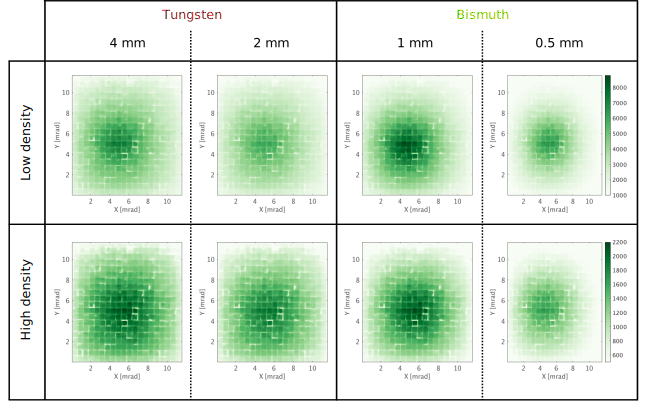
\includegraphics[trim={4.9cm 0 5cm 0}, clip, width=1.\columnwidth]{BW_GammaProfileConverter_Montage.png}

\caption[Montage of gamma profile measurements for different materials and accelerator settings.]{Montage of gamma profile images for different materials and accelerator configurations. The images on the top row are on the same colour scale, the images on the bottom respectively as well (with a maximum value of 1/4). ADD DESCRIPTION WHICH IS WHICH. TOP LOW DENSITY, BOTTOM HIGH. ALWAYS WTHICK,THIN,BITHICKTHIN, NEW ROW.}
\label{BW:figs:Gprofile_materials_montage}
\end{figure}



More specifically, $2\,\mathrm{mm}$ and $4\,\mathrm{mm}$ tungsten, $0.5$ and $1\,\mathrm{mm}$ bismuth were mounted on $0.5\,\mathrm{mm}$ plastic (PTFE), all on a motorised linear stage that allows switching between the materials or removing the converter targets from the beam path completely.
\vspace{\baselineskip}

The quantities we measure are the total counts on the gamma profile monitor (yield) and the width of the gamma signal in terms of the \textsc{fwhm} in the vertical and horizontal axis. This is being investigated for all 4 converter targets in two different electron regimes (one higher energy less charge from lower density plasma, the other higher charge but lower energy from a high density plasma). 10 shots were taken at each configuration (backing pressure A, converter 1...).


\begin{figure}
\centering
\includegraphics[trim={4.9cm 0 5cm 0}, clip, width=.9\columnwidth]{2018QED_Converter_Yield.png}
\caption[Gamma-ray yield of the bremsstrahlung source for tungsten and bismuth at different accelerator settings.]{Total measured gamma yield of the gamma-ray beam at two accelerator configurations (low and high electron densities) for tungsten (W, red) and bismuth (Bi, yellow). The values for the thin and the thick targets are shown by the thin and thick bars, respectively.}
\end{figure}


From the results we can see a couple of trends. The divergence and yield for each material is larger when the solid target is thicker, i.e. the measured gamma yield is higher for $1\,\mathrm{mm}$ of bismuth than for $0.5\,\mathrm{mm}$, and higher for $4 \,\mathrm{mm}$ than for $2\,\mathrm{mm} $of tungsten, and similarly so with respect to the divergence.
More material leads to more scattering and an increase in divergence. At the same time it indicates that more energy is converted into photons when using thicker targets.

We see that the electrons produced in a higher density plasma (higher charge, lower energy) provide a lower yield of gamma rays at higher divergences. This also appears to be sensible as the initial divergence of the electrons is higher. The yield scales quadratically with the electron energy whilst the photon number relies only linearly on the electron charge. A higher energy electron beam, even at slightly lower charge, can hence provide a higher yield (REF).

\begin{equation}
\boxed{Bremstrahlung Energy \sim Z^2 N(E) E^2}
\end{equation}
\begin{figure}
\centering
\includegraphics[trim={4.9cm 0 5cm 0}, clip, width=.9\columnwidth]{2018QED_Converter_Divergence.png}
\caption[Divergence of the gamma-ray beam for tungsten, bismuth and different accelerator settings.]{FWHM divergence of the gamma-ray beam at two accelerator configurations (low and high electron densities) for tungsten (W, red) and bismuth (Bi, yellow). The values for the thin and the thick targets are shown by the thin and thick bars, respectively. The red line indicates the field-of-view of the collimator.}
\end{figure}

Comparing the bismuth and the tungsten targets we see that the divergence for bismuth is in general lower than for tungsten. This is probably related to the thinner target. Bismuth has a higher Z-number and can provide a similar conversion efficiency at lower scattering rates.
We also observe that the yield does not increase much more from bismuth $1\,\mathrm{mm}$ to any of the tungsten targets, whilst preserving a $\sim\,10\%$ lower divergence. This indicates that most of the electrons already transferred all or a large fraction of their energy into gamma radiation and more material mainly leads to more scattering. The yield of bismuth, on the other hand, increases by around 50 percent from $0.5$ to $1\,\mathrm{mm}$ thickness. In some instances for $0.5\,\mathrm{mm}$, a faint electron signal is observed on the spectrometer screens. This confirms that somewhere around those thicknesses most of the electron energy is converted to radiation, reaching saturation.

\SMComm{How accurately is the field of view matching. Maybe run GEANT sim on the sharpness of edges.}
\EliasComm{Does this match at all? Z=74 and 83, so the ratio is 1.25, so 25 percent more yield.}

Another result can be seen in Figure \ref{BW:figs:converter_pointing}. Here the pointing stability of the gamma signal is shown. There is some scatter but most of the targets operate at a comparable level and do not show a clear trend. This makes sense, as the general pointing mainly depends on the electron pointing and should not depend on the material.

\iffalse
\begin{figure}
\centering
\includegraphics[trim={4.9cm 0 5cm 0}, clip, width=.9\columnwidth]{2018QED_Converter_YieldVDiv.png}
\caption{Gamma Profile Yield and divergence. Maybe switch to a combined plot for x and y axis.}
\label{BW:fig:converter_yield_v_div}
\end{figure}


\begin{figure}
\centering
\includegraphics[trim={4.9cm 0 5cm 0}, clip, width=.5\columnwidth]{2018QED_GConverter_PointingMM.png}\includegraphics[trim={5cm 0 5cm 0}, clip, width=.5\columnwidth]{2018QED_GConverter_PointingSigma.png}
\caption{Left: Centroid position on detector in mm, coordinate zero point is the bottom left corner of the detector. Right: Standard deviation of pointing fluctuation from mean value in mrad. This looks a bit empty. Replace this by a bar chart?}
\label{BW:figs:converter_pointing}
\end{figure}
\fi

\begin{figure}
\centering
\includegraphics[trim={4.9cm 0 5cm 0}, clip, width=.9\columnwidth]{2018QED_GConverter_Pointing.png}
\caption[Pointing of the gamma-ray beam for the different materials and accelerator settings.]{Pointing of the gamma-ray beam at two accelerator configurations (low and high electron densities) for tungsten (W, red) and bismuth (Bi, yellow). The values for the thin and the thick targets are shown by the thin and thick bars, respectively.}
\label{BW:figs:converter_pointing}
\end{figure}


\subsubsection{Throughput Collimator for Yield}

Considering the collimator and the measured divergences of the gamma rays, we can now estimate what fraction of the gamma signal that will make it through the collimator. A more divergent beam will lose more intensity but if it comes with higher yield it might still prevail.

We will use the measured \textsc{fwhm} divergence values and model the intensity profile after a Gaussian. We will also assume perfect alignment and ignore pointing for now as it is in the same ballpark for the converters and should not depend on the material.

Bismuth at $0.5\,\mathrm{mm}$ has a lower divergence and most of its energy makes it through in terms of fraction based on the initial input, followed by 1 mm bismuth. If weighed by the total flux of photons related to that converter, the higher yield of the thicker bismuth target increases the total flux. The 2 mm thick W target provides a similar throughput (in absolute numbers) as the thin bismuth target. The thicker W target reaches close to similar levels as 1 mm of bismuth but not fully.

Based on these results 1 mm bismuth appears to be the best suited candidate for this endeavour.

\begin{figure}
\centering
\includegraphics[trim={4.9cm 0 5cm 0}, clip, width=.9\columnwidth]{2018QED_AbsTransmission_V2.png}
\caption[Estimated through collimator transmitted gamma-ray yield for different materials and accelerator settings.]{Estimated transmitted yield through the collimator assuming a field of view of 7.14 mrad at two accelerator configurations (low and high electron densities) for tungsten (W, red) and bismuth (Bi, yellow). The values for the thin and the thick targets are shown by the thin and thick bars, respectively.}
\label{BW:fig:abs_transmission}
\end{figure}


\subsubsection{Noise Considerations}

The positrons produced by the BW process are detected by the timepix3 detectors. These are sensitive to gamma rays and charged particles over a wide range of energies.  The shape of the tracks in the detector allows some events to be excluded. For example, low energy charged particles produce wiggly tracks, high energy particles or gammas produce straight tracks, the length of which provides information about the angle of incidence.  As positrons transported from the collision point enter the detectors within a specific range  of angles, this can be used to exclude some high energy events.  Events which are not excluded are “candidate events”.

Gamma rays  can interact with material in the chamber (eg the magnets, the second lead collimator) and produce positrons via the BH process that have similar characteristics (energy, angle into the chicane) so that they are indistinguishable from BW positrons on the detector.  Gammas striking the vacuum windows can also scatter into the detector at the angle corresponding to a candidate event.  

 We might expect that the number of these noise events will depend on the gamma yield, the following section examines this.... 
 \vspace{\baselineskip}


When inserting the W collimator and thick W block to reduce the noise levels, the number of gamma rays that make it to the detectors is decreased significantly. This makes it more difficult to characterise how the noise at the single particle detectors (SPDs) scales as the range is limited.

Using the same setup, we are now looking at noise events reaching the SPDs, in this case only one of the TimePix detectors\footnote{Method and numbers provided by B. Kettle looking at the TimePix and finding events that look like particles, will be called clusters.}, and how it correlates with the divergence and yield of the gamma-ray signal. Our hypothesis is that a more divergent gamma-ray beam will interact with more components and apertures in the beam path, generating radiation and particles that are closely related to the BW signal and will because of this resemblance be detected by the SPDs.
\vspace{\baselineskip}

Figure \ref{BW:figs:converter_noise_div_yield} shows a plot of the total counts on the gamma detector (yield) against the number of registered particle events or `clusters' on the TimePix detector, and how the divergence is related to those noise events.

Linear trend of yield and noise on TimePix.

W data points lie on one straight line. Bi events are parallel or lower gradient, in general less noise for comparable yields.

For each material a thicker target results in more divergence. More divergence results in more noise. This confirms the need of the collimator, W block and so on and confirms the ideas behind the setup.

Looking at yield over the number of clusters, the bismuth targets perform the best when looking at fraction of flux transmitted through the collimator.
A thinner target produces less noise and bismuth provides a decent yield.

When scaling the y-axis to the absolute flux transmitted we see again that 1 mm bismuth performs similarly well as 4 mm of tungsten in terms of transmitted flux. However, we see that the ratio of yield to noise is better for bismuth due to the lower divergence.

The collimator will cut out the more divergent parts of the beam, so the noise levels will be comparable for the materials.

Looking at Figure \ref{BW:fig:Yield_with_Coll} we see that introducing the collimator cuts down the gamma yield and subsequently also the number of noise events registered on the TimePix detector. When comparing the trend of these events with the linear relations derived from the converter analysis, we see that the yield per noise further improved as we are decreasing the divergence dramatically.


\EliasComm{Need appropriate legend for all data points or combine them.}


\begin{figure}
\centering
\includegraphics[trim={4.0cm 0 5cm 0}, clip, width=.9\columnwidth]{2018QED_Converter_YieldvNoise_V2.png}
\caption[Noise versus gamma-ray yield for tungsten (W) and bismuth (Bi).]{Noise measured on the TimePix detectors as function of the yield measured on the gamma profiles for tungsten (W, red) and bismuth (Bi, yellow). The large squares indicate results from thick, the smaller ones from thin converter targets. The gradients indicate a material-dependent noise-to-yield ratio.}
\label{BW:figs:converter_noise_div_yield}
\end{figure}


\begin{figure}
\centering
\includegraphics[trim={4.0cm 0 5cm 0}, clip, width=.9\columnwidth]{2018QED_YieldvNoise_CollIN_V2.png}
\caption[Noise as a function of gamma-ray yield with the collimator in the beam path. ]{Noise as a function of gamma-ray yield with the collimator in the beam path. The noise-yield gradients for tungsten and bismuth are indicated as comparison.}
\label{BW:fig:Yield_with_Coll}
\end{figure}


\begin{figure}
\centering
\includegraphics[trim={4.9cm 0 5cm 0}, clip, width=.9\columnwidth]{2018QED_Yield_CollIN.png}
\caption[Total measured gamma yield at two accelerator configurations (low and high electron densities) for tungsten (W) and bismuth (Bi).]{Total measured gamma yield at two accelerator configurations (low and high electron densities) for tungsten (W, red) and bismuth (Bi, yellow). In turquoise the gamma yield measured using the thick bismuth target and the collimator in the beam path. The values for the thin and the thick targets are shown by the thin and thick bars, respectively.}
\label{BW:fig:Yield_with_Coll_bar}
\end{figure}


\begin{figure}
\centering
\includegraphics[trim={4.9cm 0 5cm 0}, clip, width=.9\columnwidth]{2018QED_NoiseOverYield_CollIN.png}
\caption[Fitted gradient for Noise/Yield from Figure XX at two accelerator configurations (low and high electron densities) for tungsten (W) and bismuth (Bi).]{Fitted gradient for Noise/Yield from Figure XX at two accelerator configurations (low and high electron densities) for tungsten (W, red) and bismuth (Bi, yellow). In turquoise the gradient fitted for the data using the thick bismuth target and the collimator in the beam path.}
\label{BW:fig:Yield_with_NoiseColl_bar}
\end{figure}

\subsubsection{Summary and Decision on Material}

Best flux throughput for 1 mm bismuth. Noise is also lower although the levels will change for collimator and W block conditions.
1 mm bismuth also removes all electrons and potentially reduces noise from inside the collimator (dispersed remaining electrons).

Electron regime intermediate (low density but backing pressure had to be increased due to leak). Higher energy is more preferable than a bit more charge and higher initial divergence.

In theory, even thinner target and higher Z would be favourable (as long as all electrons are converted) but Bi is the readily available material on the periodic table.

The trends confirm that we need the collimator and W block. We also see that the yield over noise improves.

\EliasComm{I estimated 50 percent loss in transmission but it looks like it is more around a factor 10. Where is this coming from? Pointing and misalignment?}
\EliasComm{Do I need to run a Monte-Carlo simulation?}


\section{Characterisation of the Gamma Signal}

\subsubsection{Yield of gamma spectrometer and profile on the different days}


\begin{figure}
\centering
\includegraphics[trim={3cm 0 5cm 0}, clip, width=.9\columnwidth]{2018QED_GSGP_Corr.png}
\caption[Linear correlation of gamma spectrometer and profile yield.]{Gamma spectrometer yield as a function of gamma profile yield for an example run. Both correlate well linearly.}
\end{figure}


\subsubsection{Detector response in experiment}

Look at the detector response in general (without corrections)

Get a better background subtraction done to avoid a fluctuation low signal tail.

Maybe make a plot of average spectra. Do they have a slight change in peak?

It seems that despite the change in spectra, the response is not changing as much.

This means the detector is not suitable to discriminate a spectrum to such detail and also is not suitable to deduce a gamma spectrum independent of assuming its shape. Luckily bremsstrahlung is well understood. It is essential to have many reference electron shots. Also a lesson for the future to take data in between.

Simulating response of detectors using GEANT.
Monoenergetic photons in a different range and present the response curves.
\vspace{\baselineskip}


Correlating Gamma profile and spec counts. No change in response for those detectors.
Seeing that this is very linear the results from gamma profile assessment are still or again valid.
This is not useful to distinguish energies.


The produced spectrum can be simulated using the electron spectra characterised earlier. GEANT. Typical gamma spectra produced are shown in FIGURE XX. 
Show that the responses for all electron spectra is fairly similar in simulations and the resulting spectra vary mostly at a low photon level and high energies.
The response of the detector only results in small variations.
\vspace{\baselineskip}

The experimental results also show only small variations which is consistent with simulations. The systematic offset is including the viewing angle, efficiency of crystals and so on.
Does the flux vary as much as the electron charge? (for the shots with W block, collimator and converter in the correlation is washed out and there is no clear indication that these things are linked). Add some plots for that as well.
Stability of gamma flux?


\begin{figure}
\centering
\includegraphics[width=.5\columnwidth]{2018QED_ElecSpecs_examples2.png}\includegraphics[width=.5\columnwidth]{2018QED_GammaSpec_simspec2.png}
\caption[Example electron spectra and corresponding in GEANT simulated gamma spectra.]{Left: Representative extreme examples of electron spectra from one day. Right: Resulting gamma spectrum based on GEANT simulations. Maybe show an average with shaded error bars instead. Add a third electron spectrum and gamma result for the other extreme.}
\end{figure}

Add the differences from day to day somewhere as well as comparison.

\begin{figure}
\centering
\includegraphics[width=.5\columnwidth]{2018QED_ElecSpecs.png}\includegraphics[width=.5\columnwidth]{2018QED_GammaSpec_simresp.png}

\includegraphics[width=.5\columnwidth]{2018QED_GammaSpec_expresp.png}\includegraphics[width=.5\columnwidth]{2018QED_GammaSpec_Average_expsim.png}

\caption{Left: Lineouts for most electron spectra. Right: Simulated detector responses. BLeft: Experimental responses. BRight: Comparison average responses.}
\end{figure}


What is the statistical variation of the signal on each day. Use the electron spectra to put a number onto this.
Use plot of relative and absolute number of photons above a threshold. Sum them up and also sum up number times energy as indicator for high energy photons.

Provide a plot with numbers on fluctuation of number of photons to expect in total and in particular above a threshold and how that varies shot-to-shot and day by day.

Provide some plots from the GEANT simulation (visualisation).

\begin{figure}
\centering
\includegraphics[trim={4.5cm 0 5cm 0}, clip, width=.9\columnwidth]{2018QED_GSpec_Variations_V2.png}

\includegraphics[trim={4.5cm 0 5cm 0}, clip, width = 0.9\columnwidth]{2018QED_GEANT_AvGSpec_V2.png}
\caption{Variations of gamma signal for the shot days. Top: Gamma-ray yield measured and relative number of photons above 400 MeV (based on GEANT simulations using the average electron spectra measured for those days). Bottom: Average gamma spectra for different shot days. Spectral shape based on GEANT simulations using average electron spectra for those days and scaled by the relative yield measured for the days.}
\end{figure}






\section{Characterisation X-ray spectra}

The analysis of the X-ray data has been conducted by Cary Colgan and Brendan Kettle (Imperial College). John Morton (AWE) provided simulations of the emitted X-ray spectra.

\begin{figure}
\centering
\includegraphics[trim={4cm 0 5cm 0}, clip, width=.9\columnwidth]{BW_XraySpec_Morton.png}

\includegraphics[trim={4cm 0 5cm 0}, clip, width=.9\columnwidth]{BW_XraySpec_AvDay.png}
\caption{X-ray spectra produced with the burn-through foil. Top: Simulated X-ray spectra for a 5 keV energy window as emitted by 100 nm germanium target heated by a high-intensity laser pulse. The y-axis indicates the number of photons per keV, the x-axis the energy of the X-ray photons (blue) and after being filtered by $5\,\mathrm{\mu m}$ of Kapton as used in the experiment (red). The dashed yellow lines indicate the spectral interval measured with the crystal spectrometer in the experiment. Bottom: X-ray spectra measured experimentally averaged for each of the three shot days A, B and C using a crystal spectrometer setup. }
\label{BW:Figs:Xray_Sim_and_Exp}
\end{figure}

The X-rays are generated by a laser beam of pulse duration $40$ ps \textsc{fwhm} heating a burn-through foil \cite{Edwards1990_BURNTHROUGH}. The target is a thin $100\,\mathrm{nm}$ coating of germanium on a $5\,\mathrm{\mu m}$-thick Kapton tape as base. The X-rays travelling to the interaction point traverse the plastic tape which results in a filtering of low energy X-rays. 
In the experiment, the X-ray source is characterised by a pinhole camera and a crystal spectrometer. The pinhole camera measures the source size and flux and the crystal spectrometer measures the spectrum of X-rays. Both diagnostics measure the X-rays from the side the foil is heated from, which means it is not filtered by the Kapton tape.
\vspace{\baselineskip}

The simulated X-ray spectrum is shown in Figure \ref{BW:Figs:Xray_Sim_and_Exp} (top) with (red) and without filtering (blue) by the tape. 
The spectrum exhibits two distinct emission peaks, one between $1.2$ and $1.5\,\mathrm{keV}$, another lower one between $1.6$ and $1.9\,\mathrm{keV}$. The spectrum underlying these two emission peaks appears to fall off exponentially from lower to higher X-ray energies, such that the emission peaks are $2-3$ orders of magnitude higher than the surrounding spectrum. When including the spectral filtering of the radiation by the layer of Kapton, most of the photons below $1\,\mathrm{keV}$ X-ray energy are cut out efficiently with exception of the spectral K-edge which leaves a narrow bandwidth at photon numbers comparable to the high emission peak.
\vspace{\baselineskip}

\begin{figure}
\centering
\includegraphics[trim={4.9cm 0 5cm 0}, clip, width=.9\columnwidth]{BW_CSpec_Pinhole_Yield.png}
\caption{X-ray yield measured with the pinhole camera (both pinholes) as a function of the yield measured with the crystal spectrometer.}
\label{BW:Figs:Xray_Pinhole_CSpec_Yield}
\end{figure}

Similarly as before we will characterise the properties of the source on the three shot days A, B and C. The average spectra measured by the crystal spectrometer for the three days are shown in Figure \ref{BW:Figs:Xray_Sim_and_Exp} (bottom). 
The spectral range indicated on the x-axis is the experimental measurement range of the crystal spectrometer and the sharp fall-off on the sides indicates the end of the camera chip or of the crystal (especially on day A). The height of the spectra is indicative of the relative X-ray yield for the different days. The distinct peaks are emission lines of the material and slight spectral shifts are due to smaller calibration and alignment errors. 
The spectral shape on day B and C are very consistent, whereas on day A the spectral lines above 1.4 keV are less pronounced and the spectrum falls off. The spectrum is also cut off at around 1.33 keV, which however is due to a misalignment in the crystal.
In general, the spectra were very consistent from shot-to-shot in terms of their spectral shape and the total yield.

\begin{figure}
\centering
\includegraphics[trim={4.9cm 0 5cm 0}, clip, width=.9\columnwidth]{BW_XraySpec_AvDay_Yield.png}
\caption{Average total X-ray yield as measured by the crystal spectrometer for the different shot days normalised by the maximum X-ray yield measured. The shot-to-shot fluctuations are negligible such that the error bars were omitted.}
\label{BW:Figs:Xray_Yield}
\end{figure}

The total yield measured by the crystal spectrometer in the limited spectral window is shown together with the yield as measured by the pinhole camera setup on the same shots in Figure \ref{BW:Figs:Xray_Pinhole_CSpec_Yield}. Both pinhole measurements agree very well with the result from the crystal spectrometer which indicates that the yield measured by the crystal spectrometer is also a good indicator for the relative changes in yield of the entire X-ray emission. From the X-ray yield it was estimated that conversion efficiency from laser light into X-rays was about 4 percent.

In Figure \ref{BW:Figs:Xray_Yield} the average X-ray yield for the three shot days is shown relative units in a bar chart. The yield was very comparable for days B and C, but was about $30\%$ lower on day A. The shot-to-shot fluctuations were negligible such that the error bars were omitted. 
This means that whilst the performance of the wakefield accelerator and as a result the gamma-ray source was better on day A, this was the opposite for the X-ray source.

\EliasComm{This might change: have to check with Cary about normalisations.}

\section{Impact of Spectral Fluctuations on the total BW cross section}

In the previous sections, we characterised the experimental fluctuations of the two photon sources for the three shot days A, B and C.

We showed that due to fluctuations in the electron beam the performance of the bremsstrahlung source fluctuates significantly from day to day. However, due to the characteristic emission spectrum of the bremsstrahlung process the fluctuations are mainly in the high energy tail of the spectrum and at low photon numbers. These high-energy gamma-rays might still be able to contribute significantly to the total number of pairs produces if their higher energy enables them to interact with a large number of low-energy photons that were not accessible on the shot days B and C.
On the other hand, we showed that the X-ray source was in general very stable from shot-to-shot and from day-to-day with respect to its spectral shape but that the total X-ray yield was by about $30\%$ lower on day A.

\begin{figure}
\centering
\includegraphics[width=.9\columnwidth]{BWD_Xsec.png}

\includegraphics[width=.9\columnwidth]{BW_Xsec_EgEx_2D.png}
\caption[Breit-Wheeler cross section for a range of X-ray and gamma-ray energies at $\theta = 140^\circ$]{Top: Total Breit-Wheeler cross section, $\sigma_{BW}$, in units of $m^{-2}$ as a function of the centre-of-mass energy, $\sqrt{s}$. Bottom: Total Breit-Wheeler cross section in $m^{-2}$ (colour scale) for an X-ray photon of energy $\epsilon_X$ (y-axis) interacting with a gamma-ray of energy $\epsilon_\gamma$ (x-axis) at an interaction angle of $\theta = 140^\circ$.}
\label{BW:Figs:Xsec_2DRange}
\end{figure}
To estimate the impact of the fluctuations in both photon sources on the number of pairs produced we have to combine both spectral measurements and calculate the Breit-Wheeler cross section, $\sigma_{BW}$ for these interactions.
The Breit-Wheeler cross section depends on the invariant mass of the collision, $s$, which incorporates the energy of the two photons involved in the interaction, $E_1$ and $E_2$ and the angle $\theta$ between them:
\begin{equation}
s = \frac{E_1 E_2 (1-\cos \theta)}{2 m^2_e c^4}.
\end{equation}

The central angle between the two photon sources was set in the experiment to be $140^\circ \pm 20^\circ$. Due to the strong collimation of the gamma-ray beam to $< 10\,\mathrm{mrad}$ the maximum spread of angles is $\theta < 0.6^\circ$ and hence negligible. The main angular spread is then contributed by the X-ray source. For now, we will, however, also ignore the angular variation of the X-ray source and calculate the cross-sections at the central crossing angle and investigate how the cross-section varies for a global change in $\theta$. 

$\sigma_{BW}$ is shown as a function of the invariant mass, $s$, in Figure \ref{BW:Figs:Xsec_2DRange} (top): $\sigma_{BW}$ is zero for $s<1$, then increases up to a peak value at $s = 2$ after which it decays slowly. Since $s \sim E_1 E_2$ or in this scenario $s \sim E_X E_\gamma$ the most likely interaction partner to produce pairs with changes with the photon energy. The higher the gamma-ray energy the lower the X-ray energy of the partner that would be most likely to produce a pair in an interaction.
In Figure \ref{BW:Figs:Xsec_2DRange} (bottom) $\sigma_{BW}$ is shown for $\theta = 140^\circ$ and a range of X-ray and gamma-ray energies accessible in this experiment. The bulk of the gamma radiation produced in the experiment was in a spectral range up to 400 MeV, which is well matched with the emission peak measured in the X-ray spectrum. The fluctuations of the gamma spectrum in the high-energy tail around 600-800 MeV on the other hand are most likely to interact with X-rays of energy $< 0.4\,\mathrm{keV}$. However, we have seen that this part of the X-ray spectrum is efficiently filtered out by the Kapton base of the burn-through foil, such that the impact of the high-energy fluctuations in the gamma-ray spectrum onto the total cross-section is suppressed.


\begin{figure}
\centering
\includegraphics[trim={4.9cm 0 5cm 0}, clip, width=0.8\columnwidth]{BWXsec_Angles_MortonRawYieldCorr.png}

\includegraphics[trim={4.9cm 0 5cm 0}, clip, width=0.8\columnwidth]{BWXsec_Angles_MortonCorrYieldCorr.png}

\includegraphics[trim={4.9cm 0 5cm 0}, clip, width=0.8\columnwidth]{BWXsec_Angles_AvDay.png}
\caption[Estimated number of pairs produced for the three shot days assuming different angles and X-ray spectra.]{With Equation \eqref{BW:Eqns:NBW} estimated number of pairs produced for the three shot days A, B and C at the interaction angles $\theta = 140^\circ \pm 20^\circ$ using the experimentally measured gamma-ray spectrum and a simulated X-ray spectrum (top), a simulated X-ray spectrum including plastic filtering (centre) and using the experimentally measured X-ray spectrum.}
\label{BW:Figs:XsecBarChart}
\end{figure}

We now estimate the average number of pairs produced evaluated for a specific day, $N_{BW,day}$, and at a fixed angle, $\theta$, by combining the spectra of the X-ray source, $\mathrm{d}N_X/\mathrm{d}E_X$, the gamma-ray spectra, $\mathrm{d}N_\gamma/\mathrm{d}E_\gamma$, and convolving it with the cross section, $\sigma_{BW}$:

\begin{equation}
\boxed{N_{BW}|_{day,\theta} \sim \int \frac{N_{ph, X}}{\mathrm{d}E_{X}} \frac{N_{ph, \gamma}}{\mathrm{d}E_{\gamma}} \sigma_{BW} (E_{X}, E_{\gamma}, \theta) \mathrm{d}E_{\gamma}\mathrm{d}E_{X}.}
\label{BW:Eqns:NBW}
\end{equation}

We calculate this for the on the three shot days experimentally measured average X-ray and gamma-ray spectra, but also consider the simulated X-ray spectra presented in Figure \ref{BW:Figs:Xray_Sim_and_Exp} to understand how much the filtering of the X-ray spectrum by the Kapton base affects the result. In addition, we consider not only the central angle $\theta = 140^\circ$ but also deviations of $\pm 20^\circ$ to estimate how a global angle changes the number of pairs produced in total but also how much deviation a spread of angles would cause.
The different values of $N_{BW}$ that were calculated for the different scenarios are presented in the bar chart in Figure \ref{BW:Figs:XsecBarChart}. The results using the simulated X-ray spectrum, scaled by the experimentally measured X-ray yield, are shown without spectral filtering in the top chart and with filtering in the chart in the centre of the Figure. The chart on the bottom shows the results using the experimentally measured X-ray spectrum. For each chart the relative number of pairs is calculated for three groups using $\theta = 140^\circ\pm20^\circ$ as interaction angle, with the height of the bars normalised to the maximum value of $N_{BW}$ within a chart.

For the case of the simulated spectrum without the plastic filter (top) the number of pairs produced for day A is the largest, followed by B and then C. This means that the higher gamma-ray yield and peak energy is outweighing the lower X-ray yield.
When including the spectral filtering of the simulated X-rays (centre) the values for days A and B equalise within errors. This indicates that the excess of pairs produced in the previous scenario are due to low-energy X-rays being able to interact with the high-energy tail of the gamma spectrum measured for day A. By removing the low-energy X-rays from the interaction days A and B equalise as the higher gamma-ray yield on day A is balanced by the higher X-ray yield of day B. The number of pairs is the lowest for day C which has an X-ray yield comparable to day B but a lower gamma-ray yield. 
Using the experimentally measured X-ray spectrum to calculate $N_{BW}$ yields similar results to the simulated X-ray spectra with the plastic filtering, which indicates that the emission line in the X-ray spectrum around $1.5\,\mathrm{keV}$ provides the most important and dominant contribution to the total production of pairs.
Across all three scenarios we see that decreasing the interaction angle, $\theta$, reduces the number of pairs produced. 

The changes in the relative number of $N_{BW}$ for the different X-ray spectra shows that we are able to mitigate the influence of the gamma-ray fluctuations by limiting which part of the X-ray spectrum is incident on the interaction point. As a result, despite significant variations in the performance of the X-ray and gamma-ray sources the relative number of photons that can in principle be produced is comparatively constant.

\section{Status of the Breit-Wheeler Analysis}

... reiterate the setup and the different components.

... emphasise that we have seen from the analysis that the gamma and X-ray sources were working...

... and that the single-particle diagnostics were working as well.

... explain that the single particle diagnostics were behaving in an expected way and we investigated their behaviour using

... the tungsten blob shots

... the magnet chicane (tracking)

... characterised magnetic chicane by using the electron beam

... noise behaviour with different blocks in.

... mention that we see a number of events on each shot based on Bethe-Heitler...

... and there are some events above that expected background

... these events are particularly visible on the 6th where the gamma conditions and the alignment was working properly.

\section{Future Work}

This analysis can be generalised into a design approach considering future measurements of the linear Breit-Wheeler mechanisms at Gemini, summarised by the three methods `stabilise, measure, mitigate'.

\EliasComm{Mention that this was not the best performance of an electron beam we are able to produce. If the spectral shape is not important we could also use shock injection. Higher energy-on target? Move target downstream and collimator?}




\subsection{Electrons}

By increasing the stability of the electron beam source we improve the stability of the gamma-ray source and our first aim should be optimising the electron source. Since we can not measure the electron beam on-shot we have to measure and characterise the electron beam fluctuations carefully before and after relevant datasets. As our gamma-ray spectrometer is also not sensitive enough to infer explicit spectral shapes without assumptions, we have to rely on a radiation process that mitigates changes in the spectral shape of the electron beam. In this case bremsstrahlung is an ideal candidate. 

\subsection{Gamma-rays}

For future experiments the bremsstrahlung source could be stabilised further by the choice of converter material. In thicker targets the energy in the gamma-ray spectrum is gradually shifted towards lower energies converting a low number of high-energy photons into many low-energy photons. This would at cost of the maximum energy and overall energy loss stabilise the radiation spectrum, but would also requrie a re-design of the magnetic chicane as the kinetic energies of the positrons produced would decrease as well. In order to measure small changes in the gamma spectrum, we have to improve the sensitivity of the gamma spectrometer setup. One proposed idea is combining the existing scintillator array with a Compton or pair spectrometer setup \cite{Lisi2018_Gamma}. As we are not able to measure small changes in the gamma spectrum we can mitigate the impact by tailoring the X-ray spectrum accordingly.

\subsection{Collimation and Shield}

\subsection{X-rays}

We choose an X-ray spectrum that is concentrated in a small energy band, here in the ML band around $1.5\,\mathrm{keV}$. The X-ray emission depends on the laser heater but is strongly determined by material properties which translate into good shot-to-shot stability. In this experiment we measured the spectral range we expected to be contributing the most to the interaction. Ideally, we would increase the measurement window with a second spectral X-ray measurement to clearly see how far the spectrum reaches. Considering the limited spectral range we can measure and the fluctuations in the gamma spectrum we can not resolve, we then mitigate the impact of both by tailoring a spectral filter such that only selected spectral components in the X-ray and gamma-ray spectrum, which we are able to measure accurately, contribute significantly to the overall production of Breit-Wheeler pairs. This will reduce the total cross-section for the interaction but mitigates the fluctuations of the sources and improves the statistical confidence in the measurement.

\section{Conclusion}

In this Chapter we presented the setup of an experimental campaign to measure the production of electron-positron pairs from the linear Breit-Wheeler process by colliding a gamma-ray beam from bremsstrahlung, using an electron beam from LWFA and a bismuth target, and X-rays from a burn-through foil driven by a high-intensity laser.

The focus of the Chapter was on the commission and optimisation of the bremsstrahlung source in terms of yield within a narrow cone of divergence and measured signal-to-noise ratio on a set of single-particle detectors by varying the material, target thickness and the accelerator setting.
The performance of the gamma-ray source was then characterised for its optimum condition across several shot days.

Electron beams from LWFA underlie intrinsic fluctuations and the performance of the accelerator can vary from day to day. The impact of these fluctuations on the properties of the radiation produced was mitigated by deciding on bremsstrahlung as mechanism. It was demonstrated that the radiation generated in the electron-solid interaction is relatively insensitive to the spectral shape of the electron beam, reducing the variations of the electron beam to fluctuations in the high energy tail of the spectrum at low photon numbers. The gamma-ray spectrometer used in this experiment was not able to resolve these fluctuations as its response is dominated by the spectral range of the bremsstrahlung spectrum containing most of the photons, which remained consistent in shape throughout the days despite the fluctuations in the electron beam.

However, we were able to mitigate the influence of the gamma-ray fluctuations by limiting the spectrum of X-rays that reaches the interaction point. By removing low-energy X-rays from the emission spectrum with a plastic filter the likeliest interaction partners of the high-energy gamma-rays the uncertainty of the fluctuations was mitigated. As a result the predicted number of pairs for the different conditions equalised.

